\documentclass{beamer}
\usepackage[utf8]{inputenc}
\usetheme{Madrid}
\usecolortheme{default}
\usepackage{amsmath,amssymb,amsfonts,amsthm}
\usepackage{txfonts}
\usepackage{tkz-euclide}
\usepackage{listings}
\usepackage{adjustbox}
\usepackage{array}
\usepackage{tabularx}
\usepackage{gvv}
\usepackage{lmodern}
\usepackage{circuitikz}
\usepackage{tikz}
\usepackage{graphicx}

\setbeamertemplate{page number in head/foot}[totalframenumber]

\usepackage{tcolorbox}
\tcbuselibrary{minted,breakable,xparse,skins}



\definecolor{bg}{gray}{0.95}
\DeclareTCBListing{mintedbox}{O{}m!O{}}{%
  breakable=true,
  listing engine=minted,
  listing only,
  minted language=#2,
  minted style=default,
  minted options={%
    linenos,
    gobble=0,
    breaklines=true,
    breakafter=,,
    fontsize=\small,
    numbersep=8pt,
    #1},
  boxsep=0pt,
  left skip=0pt,
  right skip=0pt,
  left=25pt,
  right=0pt,
  top=3pt,
  bottom=3pt,
  arc=5pt,
  leftrule=0pt,
  rightrule=0pt,
  bottomrule=2pt,
  toprule=2pt,
  colback=bg,
  colframe=orange!70,
  enhanced,
  overlay={%
    \begin{tcbclipinterior}
    \fill[orange!20!white] (frame.south west) rectangle ([xshift=20pt]frame.north west);
    \end{tcbclipinterior}},
  #3,
}
\lstset{
    language=C,
    basicstyle=\ttfamily\small,
    keywordstyle=\color{blue},
    stringstyle=\color{orange},
    commentstyle=\color{green!60!black},
    numbers=left,
    numberstyle=\tiny\color{gray},
    breaklines=true,
    showstringspaces=false,
}
%------------------------------------------------------------
%This block of code defines the information to appear in the
%Title page
\title %optional
{9.8.19}

%\subtitle{A short story}

\author % (optional)
{BALU-ai25btech11017}



\begin{document}


\frame{\titlepage}
\begin{frame}{Question}
\begin{enumerate}
    \item Two circles $x^{2}+y^{2}=6$ and $x^{2}+y^{2}-6x+8=0$ are given. 
    Then the equation of the circle through their points of intersection 
    and the point $(1,1)$ is (1980)
    \begin{enumerate}
        \item $x^{2}+y^{2}-6x+4=0$
        \item $x^{2}+y^{2}-3x+1=0$
        \item $x^{2}+y^{2}-4y+2=0$
        \item none of these
    \end{enumerate}
 \end{enumerate} 
\end{frame}
\begin{frame}{Theoretical Solution}
Let us solve the given equation theoretically and then verify the solution computationally \\
According to the question, \\
equation circles are
\begin{align}
\vec{X}^T\vec{X}-6=0\\
\vec{X}^T\vec{X}+2\myvec{-3&&0}\vec{X}+8=0
\end{align}
substute 1.1 in 1.2
\begin{align}
  \myvec{-3&&0}\vec{X}=-7\\
  x=\frac{7}{3}
\end{align}
substute 1.4 in 1.1
\begin{align}
   y=\frac{\sqrt{5}}{3},\frac{-\sqrt{5}}{3}
\end{align}
let equation of requried circle is
\end{frame}
\begin{frame}{Theoretical Solution}
\begin{align}
  \vec{X}^T\vec{X}+2\vec{u}^T\vec{X}+f=0\\
\end{align}
\begin{align}
    \myvec{2&&14&&14\\2&&\frac{2\sqrt{5}}{3}&&\frac{-2\sqrt{5}}{3}\\1&&1&&1}^T\myvec{\vec{u}\\f}=\myvec{-2\\-6\\-6}
\end{align}


\end{frame}
\begin{frame}{Theoretical Solution}
\begin{align}
   f=1\\
   \vec{u}=\myvec{\frac{-3}{2}\\0}
\end{align}
the reqiured circle equation is
\begin{align}
    x^2+y^2-3x+1=0
\end{align}
\end{frame}


\begin{frame}{Plot}
    \centering
    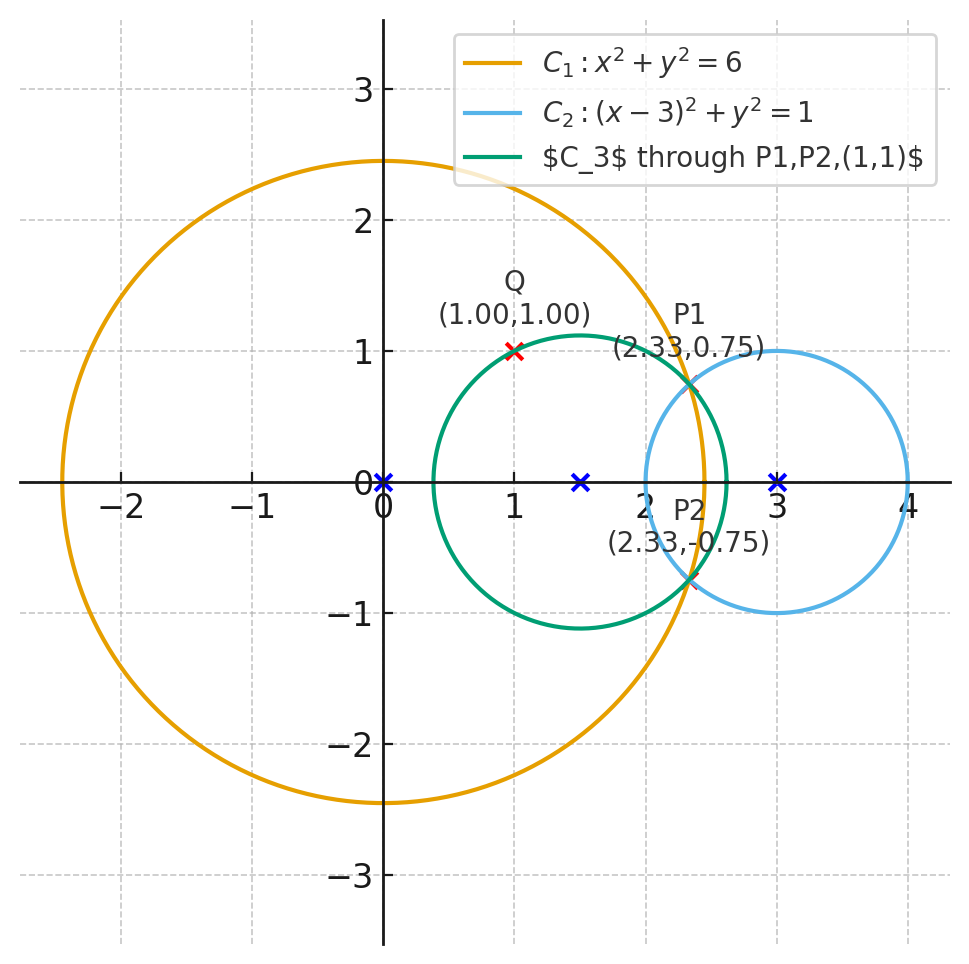
\includegraphics[width=\columnwidth, height=0.8\textheight, keepaspectratio]{figs/circles.png}     
\end{frame}
\end{document}